
\newcommand{\FigTx}{
\begin{figure*}[ht]
    \centering
    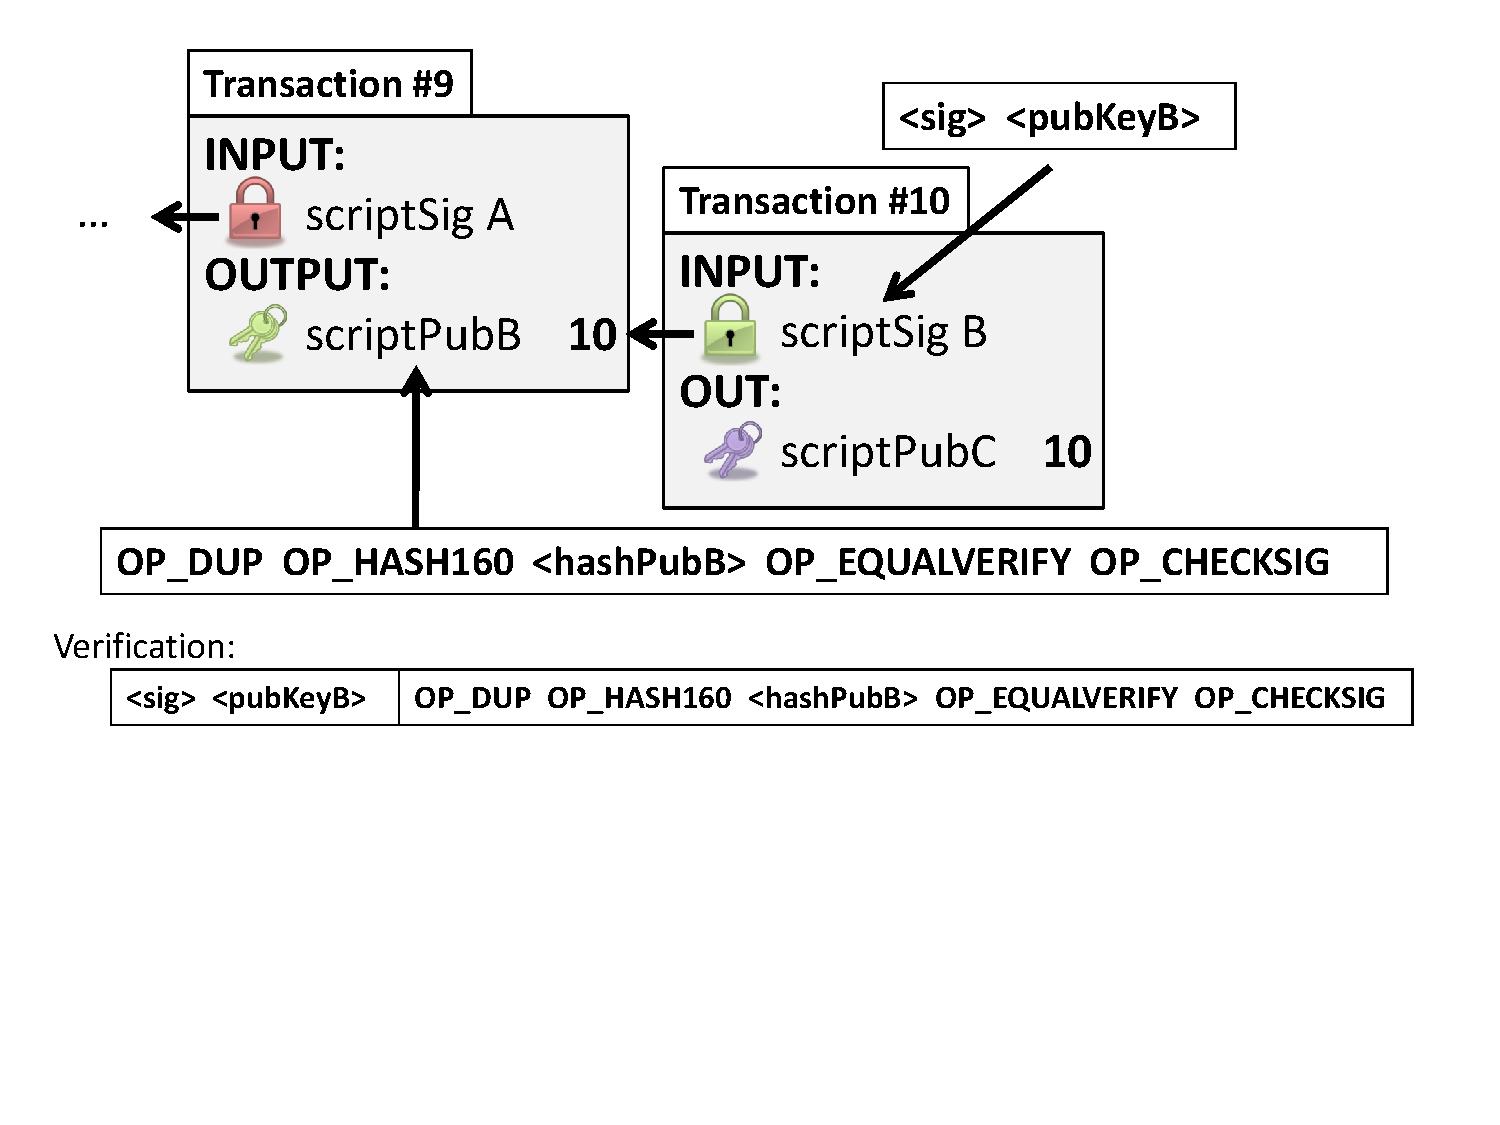
\includegraphics[width=0.9\textwidth,trim={0 6.5cm 1cm 0},clip]{btc-transaction.pdf}
    \caption{\textbf{Standard Bitcoin transaction script}\,--\, %
            Transaction \#10 spends \#9 by providing a
            valid input script that when prepended to Transaction \#9's output script,
            executes to produce a valid output. The output script stores a hash of a
            public key (verified using the OP\_DUP OP\_HASH160 and OP\_EQUALVERIFY opcodes),
            and requires a valid signature over the spending transaction (verified via
            OP\_CHECKSIG).}
    \label{fig:bitcoin-tx}
\end{figure*}
}

\newcommand{\FigOverview}{
\begin{figure*}[ht]
    \centering
    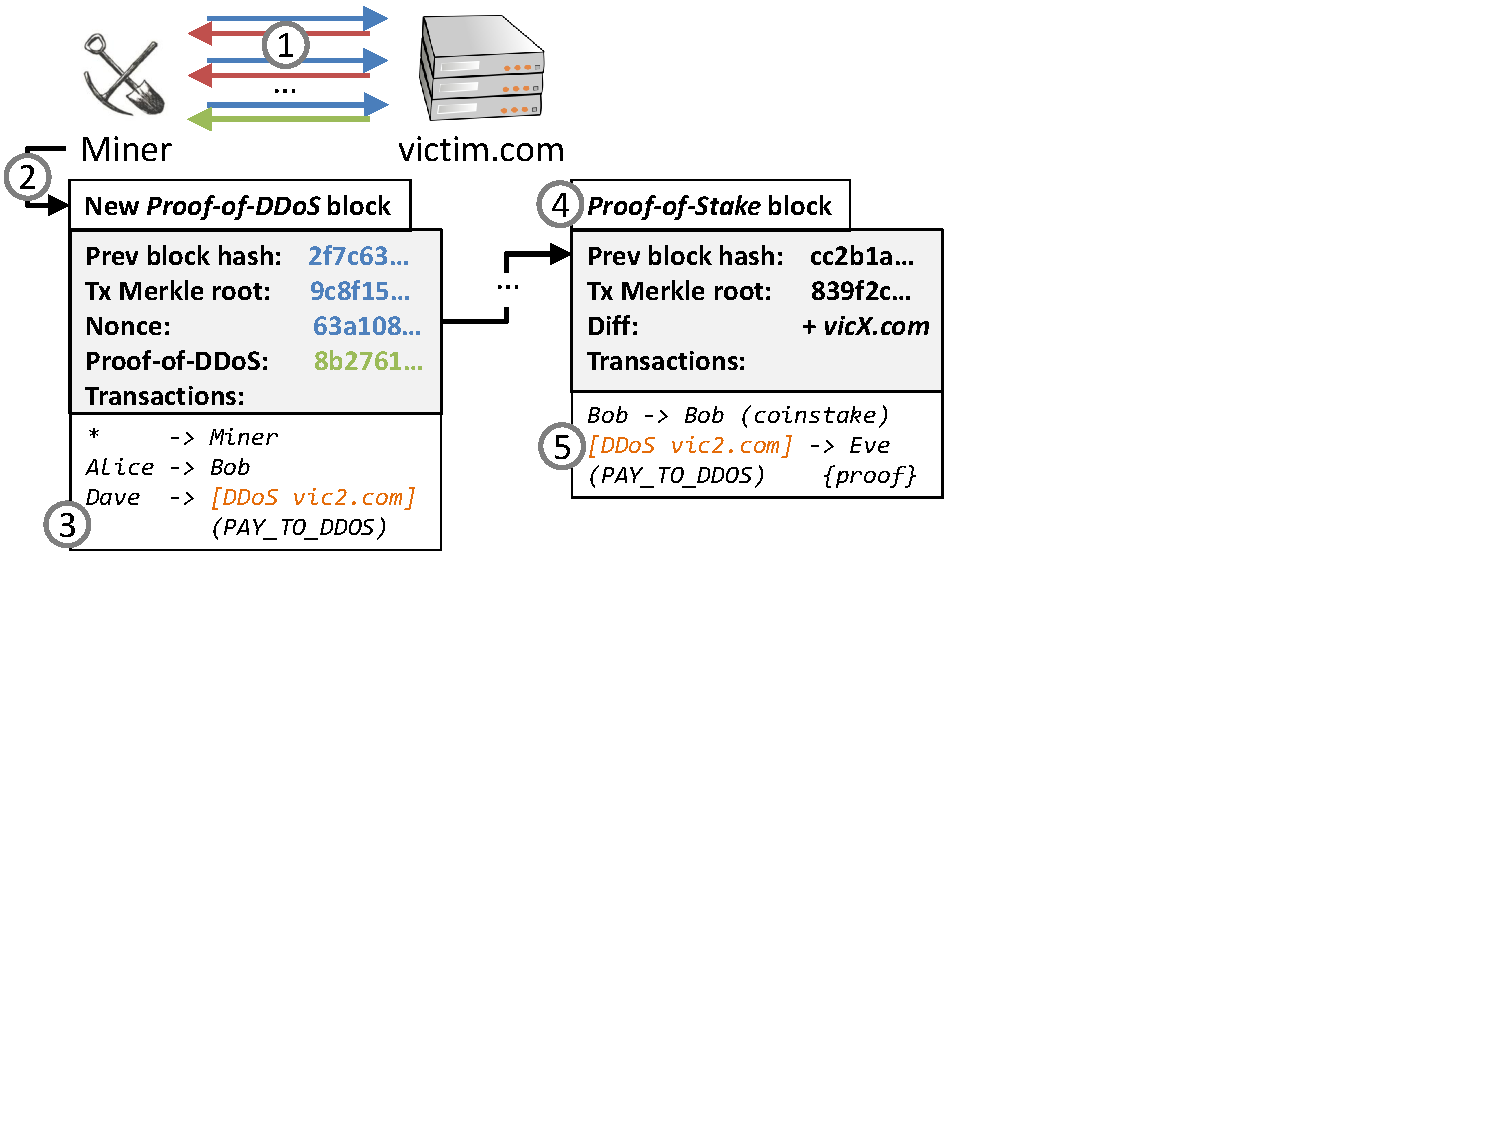
\includegraphics[width=0.9\textwidth,trim={0 9.5cm 9.2cm 0},clip]{ddoscoin-overview.pdf}
    \caption{\textbf{DDoSCoin Design}\,--\, %
    DDoSCoin miners make repeated connections to a victim server running TLSv1.2
(1). In the handshake, the miner commits to the previous block, a transaction
merkle root, and a secret nonce. Eventually the victim server will respond with
a signed message that meets the current proof-of-DDoS target, and the miner can
create a new block (2) that includes this proof. Victim targets can be selected
in one of two ways. First, participants can pay into bounties for specific
victims (3), which can be redeemed by anyone in a special PAY\_TO\_DDOS
transaction (5) if they can provide a similar proof-of-DDoS. Second, the list of
valid victims that blocks can be mined for can be updated by proof-of-stake
blocks (4).}
    \label{fig:ddoscoin-overview}
\end{figure*}
}
